\PassOptionsToPackage{dvipsnames,svgnames,table}{xcolor}
\documentclass[11pt]{article}
\usepackage[a4paper,margin=22mm]{geometry}
\usepackage[no-math]{fontspec}
\setmainfont{DejaVu Serif}
\usepackage{amsmath,amssymb,amsthm,mathtools,graphicx,xcolor,hyperref,xurl,xspace,ifthen,enumerate}
\usepackage[shortlabels]{enumitem}
\setlength{\emergencystretch}{4em}
\AtBeginDocument{\special{pdf:mapline pzdr Dingbats <uzdr.pfb}}
\SetMathAlphabet{\mathbf}{normal}{OT1}{cmr}{bx}{n}
\SetMathAlphabet{\mathbf}{bold}{OT1}{cmr}{bx}{n}
\usepackage{thmtools}
\usepackage[capitalize]{cleveref}
\newtheorem{theo}{Theorem}[section]
\newtheorem{lemm}[theo]{Lemma}
\newtheorem{thm}[theo]{Theorem}
\newtheorem{proposition}[theo]{Proposition}
\newtheorem{corollary}[theo]{Corollary}
\newtheorem{definition}[theo]{Definition}
\newtheorem{theorem}[theo]{Theorem}
\newtheorem*{remas*}{Remarks}
\newtheorem{remas}[theo]{Remarks}
\newtheorem*{exam*}{Example}
\newtheorem{ques}[theo]{Question}
\providecommand{\og}{«\nobreakspace}
\providecommand{\fg}{\nobreakspace»}
\newtheorem{lem}[theo]{Lemma}
\newtheorem{lemma}[theo]{Lemma}
\newtheorem{prop}[theo]{Proposition}
\newtheorem{coro}[theo]{Corollary}
\newtheorem{corol}[theo]{Corollary}
\newtheorem*{conj*}{Conjecture}
\newtheorem{conj}[theo]{Conjecture}
\newtheorem{conjecture}[theo]{Conjecture}
\newtheorem{Proposition}[theo]{Proposition}
\newtheorem{theoreme}[theo]{Theorem}
\theoremstyle{definition}
\newtheorem{defi}[theo]{Definition}
\newtheorem{exam}[theo]{Example}
\newtheorem{exem}[theo]{Example}
\newtheorem{remark}[theo]{Remark}
\newtheorem{example}[theo]{Example}
\newtheorem{exams}[theo]{Examples}
\newtheorem{rema}[theo]{Remark}
\newtheorem{nota}[theo]{Notation}
\newtheorem{notation}[theo]{Notation}
\newtheorem*{notas}{Notations}
\newtheorem{result}[theo]{Result}
\newtheorem{question}[theo]{Question}
\newtheorem{prob}[theo]{Problem}
\newtheorem*{rema*}{Remark}
\newtheorem*{defi*}{Definition}
\newtheorem*{theo*}{Theorem}
\newtheorem*{lemm*}{Lemma}
\newtheorem*{prop*}{Proposition}
\newcommand{\enoncename}{}
\newtheorem{corpusenonce}[theo]{\enoncename}
\newenvironment{enonce}[2][]{\renewcommand{\enoncename}{#2}\begin{corpusenonce}}{\end{corpusenonce}}
\newenvironment{enonce*}[2][]{\par\medskip\noindent\textbf{#2.}\itshape}{\par\medskip}
\newenvironment{proofc}[1][\proofname]{\begin{proof}[#1]}{\end{proof}}
\newcommand{\Mc}{\mathcal{M}}
\newcommand{\pointir}{.\ ---\ }
\newcommand{\equalenv}[2]{\expandafter\let\csname#1\expandafter\endcsname\csname#2\endcsname\expandafter\let\csname end#1\expandafter\endcsname\csname end#2\endcsname}
\providecommand{\diagbox}[3][]{\begin{tikzpicture}[x=1em,y=1em,baseline=(current bounding box.center)]\useasboundingbox(0,0) rectangle(3,1.4);\draw(0,1.4)--(3,0);\node at(.5,.3){#2};\node at(2.5,1.1){#3};\end{tikzpicture}}
\providecommand{\eg}{e.g.\ }
\providecommand{\ie}{i.e.\ }
\providecommand{\cf}{cf.\ }
\providecommand{\longthanks}[1]{\par\smallskip\noindent #1\par\smallskip}
\providecommand{\qbinom}[2]{\genfrac{[}{]}{0pt}{}{#1}{#2}}

\providecommand{\mathof}[1]{\mathrm{#1}}

\numberwithin{equation}{section}


\def\endappendix{}


\usepackage{amsmath,amssymb,amsthm,amsfonts}
\usepackage{mathtools}

\usepackage{tikz,graphicx,color}
\usepackage{tikz-cd}
\usepackage{tikz-3dplot}
\usetikzlibrary{calc}
\usetikzlibrary{arrows}
\usetikzlibrary{shapes}
\usetikzlibrary{patterns}
\usetikzlibrary{positioning}
\usetikzlibrary{arrows.meta}
\usetikzlibrary{knots}
\usetikzlibrary{decorations.markings}
\usepackage{epstopdf}

\usepackage[arrow]{xy}

\usepackage{subfig}
\usepackage{arcs}
\usepackage{xcolor}
\usepackage{tabu}
\usepackage{booktabs}

% Unused soul import omitted; no soul text-markup commands occur in retained native body.

\usepackage{letltxmacro}
\usepackage{thmtools,etoolbox}
\usepackage{nameref,hyperref}
\usepackage[capitalize]{cleveref}

\usepackage{tikz-cd}
\usepackage{xspace}

\usepackage{bm}

\newcommand\Acal{\mathcal{A}}\newcommand\Bcal{\mathcal{B}}\newcommand\Ccal{\mathcal{C}}\newcommand\Dcal{\mathcal{D}}\newcommand\Ecal{\mathcal{E}}\newcommand\Fcal{\mathcal{F}}\newcommand\Gcal{\mathcal{G}}\newcommand\Hcal{\mathcal{H}}\newcommand\Ical{\mathcal{I}}\newcommand\Jcal{\mathcal{J}}\newcommand\Kcal{\mathcal{K}}\newcommand\Lcal{\mathcal{L}}\newcommand\Mcal{\mathcal{M}}\newcommand\Ncal{\mathcal{N}}\newcommand\Ocal{\mathcal{O}}\newcommand\Pcal{\mathcal{P}}\newcommand\Qcal{\mathcal{Q}}\newcommand\Rcal{\mathcal{R}}\newcommand\Scal{\mathcal{S}}\newcommand\Tcal{\mathcal{T}}\newcommand\Ucal{\mathcal{U}}\newcommand\Vcal{\mathcal{V}}\newcommand\Wcal{\mathcal{W}}\newcommand\Xcal{\mathcal{X}}\newcommand\Ycal{\mathcal{Y}}\newcommand\Zcal{\mathcal{Z}}

\newcommand\abf{\mathbf{a}}\newcommand\bbf{\mathbf{b}}\newcommand\cbf{\mathbf{c}}\newcommand\dbf{\mathbf{d}}\newcommand\ebf{\mathbf{e}}\newcommand\fbf{\mathbf{f}}\newcommand\gbf{\mathbf{g}}\newcommand\hbf{\mathbf{h}}\newcommand\ibf{\mathbf{i}}\newcommand\jbf{\mathbf{j}}\newcommand\kbf{\mathbf{k}}\newcommand\lbf{\mathbf{l}}\newcommand\mbf{\mathbf{m}}\newcommand\nbf{\mathbf{n}}\newcommand\obf{\mathbf{o}}\newcommand\pbf{\mathbf{p}}\newcommand\qbf{\mathbf{q}}\newcommand\rbf{\mathbf{r}}\newcommand\sbf{\mathbf{s}}\newcommand\tbf{\mathbf{t}}\newcommand\ubf{\mathbf{u}}\newcommand\vbf{\mathbf{v}}\newcommand\wbf{\mathbf{w}}\newcommand\xbf{\mathbf{x}}\newcommand\ybf{\mathbf{y}}\newcommand\zbf{\mathbf{z}}

\newcommand\C{\mathbb{C}}
\newcommand\R{\mathbb{R}}
\newcommand\N{\mathbb{N}}
\newcommand\Z{\mathbb{Z}}
\newcommand\Q{\mathbb{Q}}

\newcommand\Ahat{\hat{A}} 
\newcommand\ipar{{(i)}}
\newcommand\parr[1]{{({#1})}}


\newcommand\m{{\mu}}
\newcommand\lm{{\l/\m}}

\newcommand\Id{\operatorname{Id}}
\newcommand\Vol{\operatorname{Vol}}
\newcommand\diag{{ \operatorname{diag}}}
\newcommand\rank{{ \operatorname{rank}}}
\newcommand\rk{{\mathrm{rank}}}
\newcommand\cork{ \operatorname{corank}}
\newcommand\corank{ \operatorname{corank}}
\newcommand\codim{ \operatorname{codim}}
\newcommand\op{{ \operatorname{op}}}
\newcommand\sh{{ \operatorname{sh}}}
\newcommand\Conv{ \operatorname{Conv}}
\newcommand\Span{ \operatorname{Span}}
\newcommand\proj{ \operatorname{proj}}
\newcommand\sgn{ \operatorname{sgn}}
\newcommand\wt{\operatorname{wt}}
\newcommand\inv{\operatorname{inv}}
\newcommand\Int{\operatorname{int}}
\newcommand\Cone{\operatorname{Cone}}

\newcommand\GL{\operatorname{GL}}
\newcommand\SL{\operatorname{SL}}
\newcommand\Mat{\operatorname{Mat}}
\newcommand\Gr{\operatorname{Gr}}
\newcommand\Grtnn{\Gr_{\ge 0}}
\newcommand\Grtp{\Gr_{>0}}
\newcommand\alt{\operatorname{alt}}
\newcommand\Mattp{\operatorname{Mat}_{>0}}
\newcommand\Mattnn{\operatorname{Mat}_{\ge0}}


\newcommand\Bound{{\rm Bound}}

\newcommand\af{{\rm af}}
\newcommand\Inv{{\rm Inv}}

\newcommand\id{{\operatorname{id}}}

\newcommand\xs{\operatorname{xs}}
\newcommand\ys{\operatorname{ys^{-1}}}
\newcommand\bs{\backslash}
\newcommand\oPi{\accentset{\circ}{\Pi}}
\newcommand\bt{{\mathbf{t}}}
\newcommand\bw{{\mathbf{w}}}
\newcommand\bv{{\mathbf{v}}}
\newcommand\bu{{\mathbf{u}}}
\newcommand\ba{{\mathbf{a}}}
\newcommand\bb{{\mathbf{b}}}
\newcommand\bc{{\mathbf{c}}}
\newcommand\geqJ{\succeq}
\newcommand\gessJ{\succ}

\newcommand\bx{{\bm{x}}}
\newcommand\by{{\bm{y}}}
\newcommand\bi{{\mathbf{i}}}
\newcommand\bj{{\mathbf{j}}}




\newcommand\Deltamp{\Delta^\mp}
\newcommand\Deltapm{\Delta^\pm}


\newcommand\RedMR{\operatorname{Red}}
\newcommand\Red{\operatorname{Red}}
\newcommand\weightL{Y(T)}
\newcommand\rootL{Q_\Phi}
\newcommand\Qkls{Q_P(W,W_J)}


\newcommand\chr{\operatorname{char}}

\let \oldlabel \label
\let\oldref\ref
\let\oldcref\cref





\newcommand\B{{\mathcal B}}
\newcommand\G{\Gcal}
\newcommand\Caff{{\mathcal{C}}}
\newcommand\GCMaff{\tilde{A}}

\newcommand\Phiaff{\Delta}
\newcommand\re{\operatorname{re}}
\newcommand\im{\operatorname{im}}
\newcommand\Phire{\Phiaff_{\re}}
\newcommand\Phiim{\Phiaff_{\im}}

\newcommand\FPS{{\mathcal{A}}}
\newcommand\CRL{{\rootL^\vee}}
\newcommand\minn{{\operatorname{min}}}
\newcommand\Cast{\C^\ast}

\newcommand\tauk{\tau_k}
\newcommand\leqop{\leq^\op}
\newcommand{\Povar}{\mathring{\Pi}}

\newcommand\Boundkn{\operatorname{Bound}(k,\n)}


\newcommand\BAcomb{\psi}
\newcommand\BAgeom{\bar\varphi_u}
\newcommand\BAgeo{\varphi_u}

\newcommand\tht{t}





\newcommand\Ng{{N_g}}
\newcommand\strix{t_1(x)}
\newcommand\strixn{t_1(x_n)}
\newcommand\Bcl{\overline{B}}
\newcommand\epsb{\eps_B}


\newcommand\conept{c}

\newcommand\Link{\operatorname{Lk}}

\newcommand\eps{\varepsilon}






\newcommand\Spec{\operatorname{Spec}}

\newcommand\pr{^{\parr{r}}}

\newcommand\om{\omega}
\newcommand\pan{^\parr{n}}

\newcommand*{\smallcap}{{\mathbin{\scalebox{0.5}{\ensuremath{\cap}}}}}

\newcommand\gc{g_\smallcap}
\newcommand\BG{B_-\backslash G}
\newcommand\BGtnn{(B_-\backslash G)_{\geq0}}

\newcommand\GBsf{(G/B_-)(K)}
\newcommand\BGsf{(\BG)(K)}


\newcommand\str{\operatorname{str}}
\newcommand\strd{\operatorname{str}^\ast}

\newcommand\Sn{S_\n}
\newcommand\chiv{\vec\chi_{v}}

\newcommand\chiw{\vec\chi^{\,w}}
\newcommand\chiww{\vec\chi^{\,{\ww}}}

\newcommand\flec{\vec f}
\newcommand\fR{\vec f}


\newcommand\Ztnn{\Z_{\geq0}}


\newcommand\colspan{\operatorname{ColumnSpan}}

\newcommand\Qkn{Q_{k,\n}}
\newcommand\Bkn{\Boundkn}
\newcommand\Skn{S_\n^{(k)}}

\newcommand\perm{\operatorname{perm}}
\newcommand\Lperm{L^{\perm}}
\newcommand\tor{\operatorname{tor}}
\newcommand\Ltor{L^{\tor}}
\newcommand\grid{\operatorname{grid}}
\newcommand\Lgrid{L^{\grid}}
\newcommand\Lgridt{\tilde L^{\grid}}
\newcommand\rich{\operatorname{Rich}}
\newcommand\Lrich{L^{\rich}}
\newcommand\plab{\operatorname{plab}}
\newcommand\Lplab{L^{\plab}}
\newcommand\cox{\operatorname{Cox}}
\newcommand\Lcox{L^{\cox}}

\newcommand\fp{\pi}


\newcommand\pig{\pi_G}

\newcommand\Arg{\operatorname{arg}}

\newcommand\ice{\operatorname{ice}}
\newcommand\QG{Q_G}
\newcommand\Qice{\widetilde{Q}}
\newcommand\QGice{\Qice_G}

\newcommand\BQ{B(Q)}
\newcommand\BQice{\widetilde{B}(\Qice)}
\newcommand\Vice{\widetilde{V}}

\newcommand\AQ{\Acal(Q)}
\newcommand\AQG{\Acal(\QG)}
\newcommand\AQGice{\Acal(\QGice)}
\def\RQ(#1){R(Q;#1)}
\def\RQX#1#2{R(#1;#2)}
\def\RQice(#1){R(\Qice;#1)}
\def\RQG(#1){R(\QG;#1)}
\newcommand\F{\mathbb{F}}

\newcommand\Pio{\Pi^\circ}
\newcommand\HOMP{P}
\newcommand\unknot{
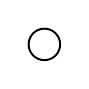
\begin{tikzpicture}[baseline=(ZUZU.base),scale=0.2]\coordinate(ZUZU) at (0,-0.6);
\draw[line width=0.7pt] (0,0) circle (1cm);
  \end{tikzpicture}
}


\newcommand\Top{{\operatorname{top}}}
\def\Ptop_#1(#2){P^\Top(#1;#2)}

\newcommand\fbar{\bar f}
\newcommand\taukn{\tau_{k,\n}}
\newcommand\T{\mathbb{T}}

\newcommand\Cproj{\overline{C}}


\newcommand\fro{\operatorname{fro}}
\newcommand\mut{\operatorname{mut}}
\newcommand\Vfro{V_{\fro}}
\newcommand\Vmut{V_{\mut}}
\newcommand\bip{\operatorname{bip}}
\newcommand\Gbip{G^{\bip}}



\def\Qicefr[#1]{\Qice[#1]}
\newcommand\Bice{\widetilde{B}}
\newcommand\bice{\tilde{B}}
\newcommand\XQice{\Xcal(\Qice)}
\newcommand\XBQice{\Xcal(\BQice)}
\newcommand\AX{\Acal}
\newcommand\AQice{\Acal(\Qice)}
\newcommand\ABQice{\Acal(\BQice)}

\newcommand\chiQ{\chi_Q}
\newcommand\chiQice{\chi_{\Qice}}

\newcommand\Gm{\F^\ast}
\newcommand\Ga{\F}


\newcommand\Aut{\operatorname{Aut}}
\def\QX(#1){Q_{#1}}
\newcommand\disjun{\sqcup}
\newcommand\pmi{\pm I}
\newcommand\pmim{(\pmi)^m}

\newcommand\pmn{\pm I}
\newcommand\pmnm{(\pmn)^m} 
\newcommand\DRW{(\pmn)^m} 

\newcommand\Gbw{G(\bw)}
\def\GX(#1){G(#1)}

\newcommand\rev{\operatorname{rev}}


\newcommand\rowspan{\operatorname{RowSpan}}

\def\figref#1(#2){Figure~\hyperref[#1]{\ref*{#1}(#2)}}

\newcommand\conn{\operatorname{c}}
\newcommand\ncyc{\conn}

\newcommand\n{N}
\newcommand\qq{q^{\frac12}}
\newcommand\qqi{q^{-\frac12}}

\newcommand\disk{\mathbf{D}}

\newcommand\Lrichp{L}

\newcommand\projt{p_{\T}}
\def\projtx#1{\overline{#1}}

\newcommand\Louise{locally acyclic\xspace}
\newcommand\Louiseleaf{recurrent leaf\xspace} 


\newcommand\degtop{\deg^{\Top}}
\newcommand\tI{{\tilde I}}
\newcommand\pmtI{\pm\tI}
\def\linkurl#1{\textup{\texttt{\href{http://katlas.org/wiki/#1}{#1}}}}
\newcommand\comma{} 

\newcommand\Btilde{$\tilde{\text{B}}$}



\def\hopflink{
\scalebox{0.3}{
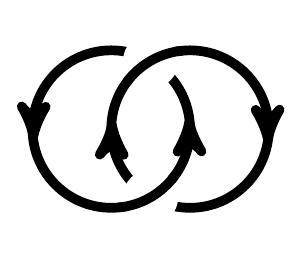
\begin{tikzpicture}[baseline=(ZUZU.base)]\coordinate(ZUZU) at (0,-0.8);
\draw[line width=3.5pt, white,
    decoration={markings,mark=at position 0 with {\arrow[scale=1,black]{stealth'}}},
    decoration={markings,mark=at position 1 with {\arrow[scale=1,black]{stealth'}}},
    postaction={decorate}] (-0.99,-0.15)--(-1,-1)--(1,-1)--(0.99,0.15);
\draw[line width=3.5pt, white,
    decoration={markings,mark=at position 0.01 with {\arrow[scale=1,black]{stealth'}}},
    decoration={markings,mark=at position 0.99 with {\arrow[scale=1,black]{stealth'}}},
    postaction={decorate}] (1.99,-0.15)--(2,-1)--(0,-1)--(0.01,0.15);
\begin{knot}[
    clip width=6,
    flip crossing={1},
    ]
    \strand [line width=3.5pt] (0,0) circle (1.0cm);
    \strand [line width=3.5pt] (1,0) circle (1.0cm);
\end{knot}
\end{tikzpicture} 
}
}

\newcommand\pikn{\pi_{k,\n}}
\newcommand\fkn{f_{k,\n}}


\newcommand\pA{^{(1)}}
\newcommand\pB{^{(2)}}
\newcommand\pC{^{(3)}}
\newcommand\pD{^{(4)}}
\newcommand\pE{^{(5)}}
\newcommand\red{-}
\newcommand\Qred{Q^{\red}}
\newcommand\QredG{Q^{\red}_G}
\newcommand\BQredG{B(\QredG)}

\newcommand\E{H}
\newcommand\Tc{{T,c}}

\newcommand\mysq{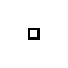
\begin{tikzpicture}
\node[draw=black,line width=1pt, rectangle,scale=0.5,fill=white] (A) at (0,0) {};
\end{tikzpicture}}

\newcommand\tils{\tilde s}


\newcommand\HHH{H\!\!H\!\!H}
\newcommand\HHHC{\HHH_\C}
\newcommand\PGL{\operatorname{PGL}}

\def\mirr#1{#1^\ast}
\newcommand\Divide{\Delta}

\newcommand{\FLY}{HOMFLY\xspace}
\newcommand{\la}{\lambda}
\newcommand{\w}{{\mathbf{w}}}
\newcommand{\pt}{{\rm pt}}
\newcommand{\arxiv}[1]{\href{https://arxiv.org/abs/#1}}



















\begin{document}
\section*{\raggedright 839: Recurrent-leaf strata of really-full-rank cluster varieties split as an affine line times a rank-reduced variety over any field}
\noindent\textbf{Author:} Galashin, Pavel; Lam, Thomas\par\noindent\textbf{Source:} Plabic links, quivers, and skein relations. Algebraic Combinatorics 7 (2024), publisher version, DOI 10.5802/alco.345. \url{https://alco.centre-mersenne.org/articles/10.5802/alco.345/}
\par\noindent\textbf{License:} CC BY 4.0, \url{https://creativecommons.org/licenses/by/4.0/}. The original publisher PDF cover has the explicit license notice. See the saved source/license records.
\par\noindent\textbf{Editorial material note (not author text):} The selected problem is Proposition5.14 over the exact arbitrary field, really-full-rank ice quiver and recurrent-leaf hypothesis. Full author quiver/cluster definitions and the complete frozen-row reduction, primitive torus orbit transversal and reduced exchange-matrix construction are retained. Named Muller localization/cover and Lam--Speyer cluster automorphism facts remain explicit standard references. The later leaf point-count corollary is unselected context. Standalone section/shared theorem counters preserve the original printed5.14 locator; references to unrelated original illustrations or HOMFLY context retain their printed article numbers. The unused Povar helper has no actual retained body uses. No mathematical construction or proof is supplied by an editor. All proof text and formulas below are editable author TeX. Mathematical wording, language and proof order are retained. Only the article class, title matter and bibliography presentation are adapted for independent compilation; no proof has been generated or repaired.
\par\noindent\textbf{Editorial difficulty:} H2: The proof localizes the cluster algebra at the neighbouring variable, isolates a primitive frozen-torus action by integral row operations, proves each orbit meets a prescribed monomial fibre once, and constructs the resulting really-full-rank exchange matrix. This explicit geometric reduction is nonroutine and keeps the recurrent-leaf/full-rank assumptions.
\medskip\hrule\medskip
\noindent\textbf{Author statement, complete proof and local supporting text follow in source order.}
\newtheorem{problem}[theo]{Problem}
%\equalenv{example}{exam}
%\equalenv{notation}{nota}

\crefname{figure}{Figure}{Figures}
\crefname{conjecture}{Conjecture}{Conjectures}
%\equalenv{conjecture}{conj}

\addtotheorempostheadhook[theorem]{\crefalias{theoremlisti}{theorem}}
\addtotheorempostheadhook[lemma]{\crefalias{theoremlisti}{lemma}}
\addtotheorempostheadhook[proposition]{\crefalias{theoremlisti}{proposition}}
\addtotheorempostheadhook[corollary]{\crefalias{theoremlisti}{corollary}}

\setcounter{section}{4}
\section{Quivers}
In this section, we introduce the point count polynomial $R(Q;q)$ of a \Louise %
 quiver, and study its basic properties.  We use this polynomial to define the \emph{$Q$-Catalan number} of $Q$, an integer that we conjecture to be nonnegative in \cref{conj:Catalan}. We refer the reader to~\cite{FWZ_book} for an excellent introduction to quivers and cluster algebras.

\subsection{Quiver mutation}\label{sec:quiver}
Recall that a \emph{quiver} is a directed graph without directed cycles of length $1$ and $2$.

Given a quiver $Q$ and a vertex $j\in V(Q)$, one can define another quiver $Q'=\mu_j(Q)$ called the \emph{mutation of $Q$ at $j$}. This operation preserves the set of vertices:  $V(Q')=V(Q)$, and changes the set of arrows as follows:
\begin{itemize}
\item for every length $2$ directed path $i\to j\to k$ in $Q$, add an arrow $i\to k$ to $Q'$;
\item reverse all arrows in $Q$ incident to $j$;
\item remove pairs of opposite arrows (i.e.  directed $2$-cycles) in the resulting directed graph, one pair at a time, until no such pairs are present.
\end{itemize}

An \emph{ice quiver} is a quiver $\Qice$ whose vertex set $\Vice=V(\Qice)$ is partitioned into \emph{frozen} and \emph{mutable} vertices: $\Vice=\Vfro\sqcup \Vmut$. We automatically omit all arrows in $\Qice$ both of whose endpoints are frozen. For an ice quiver $\Qice$, its \emph{mutable part} is the induced subquiver of $\Qice$ with vertex set $\Vmut$.  %
 For a set $S\subset \Vmut$, let $\Qicefr[S]$ denote the ice quiver obtained from $\Qice$ by further declaring all vertices in $S$ to be frozen. We write $\Qice-S$ for the ice quiver obtained from $\Qice$ by removing the vertices in $S$.  For a simply-laced Dynkin diagram $D$, we say that $Q$ or $\Qice$ has type $D$, or is a $D$-quiver, if the underlying graph of $Q$ is isomorphic to $D$.


 Let $\Qice$ be an ice quiver with $\Vice=[n+m]$, $\Vmut=[n]$, and $\Vfro=[n+1,n+m]:=\{n+1,n+2,\dots,n+m\}$. We represent it by an $(n+m)\times n$ \emph{exchange matrix} $\BQice=(b_{ij})$, defined by
 \begin{equation*}%
   b_{ij}=\#\{\text{arrows $i\to j$ in $\Qice$}\} - \#\{\text{arrows $j\to i$ in $\Qice$}\}.
 \end{equation*}
The top $n\times n$ submatrix $\BQ$ of $\BQice$ is skew-symmetric, and is called the \emph{principal part} of $\BQice$.  
%

%
%
%
%
%
%
%
%
%
%
%
%
%
%
%
%
 
%

Let $\Bice$ be an $(n+m)\times n$ matrix. We denote $\cork(\Bice):=n-\rk(\Bice)$. Following~\cite{LS}, we say that an $(n+m)\times n$ matrix $\Bice$ is \emph{really full rank} if the rows of $\Bice$ span $\Z^n$ over $\Z$. We say that $\Qice$ is \emph{really full rank} if $\BQice$ is really full rank, and write $\cork(\Qice):=\cork(\BQice)$.   We say that $\Qice$ is \emph{torsion-free} if the abelian group $\Z^{n+m}/\BQice \Z^n$ is torsion-free, equivalently, if $\Z^n/\BQice^T \Z^{n+m}$ is torsion-free.  Thus, $\Qice$ is really full rank if and only if it is both full rank and torsion-free.

\begin{definition}
Given a quiver $Q$, we say that an ice quiver $\Qice$ with mutable part $Q$ is a \emph{minimal extension} of $Q$ if $\Qice$ has $m=\cork(Q)$ frozen vertices and is really full rank.
\end{definition}

\begin{lemma}\label{lem:ext}
If $Q$ is torsion-free then it admits a minimal extension.
%
\end{lemma}
\begin{proof}
If $Q$ is torsion-free, we can find vectors $d_1,\ldots,d_m \in \Z^n$ that form a basis of $\Z^n/B(Q)^T \Z^n$.  Define $\Qice$ with $m$ frozen vertices so that the bottom $m$ rows of the exchange matrix $\Bice$ are equal to $d_1,\ldots,d_m$.
\end{proof}
%
%

\begin{example}
The exchange matrices of the two quivers $Q,Q'$ in \figref{fig:LA}(c) are given by
$$
\BQ=\begin{pmatrix}
0 & 2 & -2 \\
-2&0&2\\
2&-2&0
\end{pmatrix} \qquad \text{and} \qquad
B(Q')=\begin{pmatrix}
0 & -1& -1 &2 \\
1&0&1 &-1\\
1&-1&0 &-1 \\
-2&1&1&0
\end{pmatrix}.
$$
Thus, $\cork(Q)=1$, $\cork(Q')=0$, and neither quiver is torsion-free.
\end{example}

We say that an ice quiver $\Qice$ is \emph{isolated} if it has no arrows. For example, the quiver in Figure~8(c) is isolated.

We call an ice quiver $\Qice$ \emph{acyclic} if it has no directed cycles, and \emph{mutation acyclic} if it is mutation equivalent to an acyclic ice quiver.  For example, any quiver of Dynkin type is acyclic, as is the quiver in \figref{fig:LA}(a).  The quiver in Figure~8(a) and the left quiver in \figref{fig:LA}(b) are not acyclic, but they are both mutation acyclic, since mutating a single vertex in each of these quivers makes them acyclic.

An edge $u\to v$ in a quiver $Q$ is called a \emph{separating edge}~\cite{Muller} if it does not belong to a bi-infinite walk in $Q$. Here, a \emph{bi-infinite walk} is a sequence $(w_j)_{j\in\Z}$ of vertices in $Q$ such that for each $j\in\Z$, $Q$ contains an arrow $w_j\to w_{j+1}$.

We define the class of \emph{\Louise quivers}, called ``Louise" in \cite{MSLA,LS}, as follows.
\begin{itemize}
\item Any isolated quiver $Q$ is \Louise.
\item Any quiver that is mutation equivalent to a \Louise quiver is \Louise.
\item Suppose that a quiver $Q$ has a separating edge $u\to v$, and that all three quivers $Q-\{u\}$, $Q-\{v\}$, $Q-\{u,v\}$ are \Louise. Then $Q$ is \Louise.
\end{itemize}
We say that an ice quiver $\Qice$ is \emph{\Louise} if its mutable part $Q$ is \Louise.    See \cref{fig:LA}.
\begin{figure}
  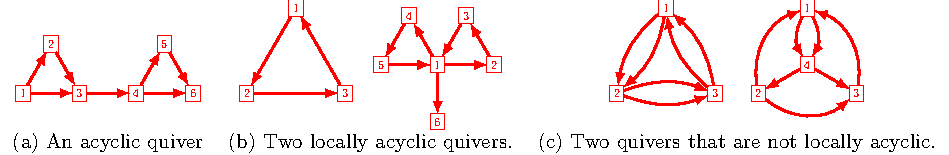
\includegraphics[width=\textwidth]{../assets/839/Louise.pdf}
  \caption{\label{fig:LA} Acyclic, locally acyclic and non-\Louise quivers.}
\end{figure}

\subsection{Cluster algebras}
Let $\Qice$ be an ice quiver with $\Vice=[n+m]$, $\Vmut=[n]$, and $\Vfro=[n+1,n+m]$.  We associate to $\Qice$ the initial seed $(x_1,x_2,\ldots,x_{n+m})$ of \emph{cluster variables}, considered as elements in the function field $\Fcal = \Q(x_1,x_2,\dots,x_{n+m})$.  The variables $x_{n+1},\ldots,x_{n+m}$ are called \emph{frozen variables}.  For a mutation $Q' = \mu_j(Q)$, we associate the seed $(x'_1,x'_2,\ldots,x'_{n+m})$, where $x'_i = x_i$ if $i \neq j$ and one has the new cluster variable
$$
x'_j = \frac{\prod_{r \to j} x_r + \prod_{j \to s} x_s}{x_j} \in \Fcal.
$$
By repeatedly mutating, we generate (possibly infinitely) many seeds and cluster variables. 
 We denote by $\AQice=\ABQice$ the cluster algebra associated to $\Qice$. This is the $\Z$-subalgebra of $\Q(x_1,x_2,\dots,x_{n+m})$ generated by all cluster variables and the inverses of frozen variables. 
 
The \emph{cluster variety} $\XQice=\XBQice$ is defined to be the scheme
\begin{equation*}%
\XQice:=\Spec(\AQice).
\end{equation*}
We say that $\AQice$ (resp. $\XQice$) is a cluster algebra (resp. cluster variety) \emph{of type $Q$}, where $Q$ is the mutable part of $\Qice$.  We say that $\AQice$ is isolated, acyclic, (really) full rank, if $\Qice$ is isolated, mutation acyclic, (really) full rank, respectively.  If $\Qice$ is a \Louise quiver, then $\AQice$ is locally acyclic in the sense of Muller~\cite{Muller}.


\begin{proposition}[{\cite[Theorem 7.7]{Muller}, \cite[Theorem 10.1]{LS}}]\label{prop:Mulsmooth}
Suppose that $\Qice$ is \Louise and really full rank.  Then $\XQice_\C$ is a smooth complex algebraic variety and $\XQice_{\bar \F_q}$ is smooth for any prime power $q$.
\end{proposition}

\begin{proposition}[{\cite[Corollary 5.4]{Muller}}]\label{prop:Mulcover}
Let $i \to j$ be a separating edge in $\Qice$.  Then the open sets $\{x_i \neq 0\}$ and $\{x_j \neq 0\}$ cover $\XQice$.
\end{proposition}

\begin{proposition}[{\cite[Proposition 3.1, Lemma 3.4, Theorem 4.1]{Muller}}]\label{prop:Mulloc}
Suppose that $i \in V(\Qice)$ is a mutable vertex such that $Q- \{i\}$ is \Louise.  Then $\AQice[x_i^{-1}] \simeq \AX(\Qice[i])$.
\end{proposition}

\subsection{Quiver point count}
For a mutable quiver $Q$, we define the function $\RQ(q)$ as follows. Choose a really full rank ice quiver $\Qice$ with mutable part $Q$ and $m$ frozen vertices. Then for $q$ a prime power, we set
\begin{equation}\label{eq:RQ_dfn}
  \RQ(q):=\frac{\#\XQice(\F_q)}{(q-1)^m}.
\end{equation}
For a rational function $R(q)=P(q)/Q(q)$, we let the \emph{degree} $\deg(R)$ be the difference $\deg(P)-\deg(Q)$. 
\begin{proposition}[{\cite[Proposition 5.11 and Theorem 10.5]{LS}}]\label{prop:Q_pcnt}
  Let $Q$ be a quiver with $n$ vertices.
  \begin{enumerate}
  \item The function $\RQ(q)$ defined in~\eqref{eq:RQ_dfn} does not depend on the choice of $\Qice$.
  \item Suppose $Q$ is \Louise. Then $\RQ(q)$ is a rational function in $q$ of degree $n$. %
  \end{enumerate}
\end{proposition}
If $u \to v$ is a separating edge in $Q$ and $Q-\{u\},Q-\{v\},Q-\{u,v\}$ are \Louise, then we have the recurrence
\begin{equation}\label{eq:RQ_recurrence}
  \RQ(q) = (q-1)\RQX{Q-\{u\}}{q}+ (q-1)\RQX{Q-\{v\}}{q}- (q-1)^2\RQX{Q-\{u,v\}}{q},
\end{equation}
which follows from Propositions~\ref{prop:Mulcover} and~\ref{prop:Mulloc}.

\begin{proposition}[{\cite[Proposition 3.9]{LS2}}] \label{prop:acycliccount}
Let $Q$ be an acyclic quiver with $n$ vertices.  Then 
$$
\RQ(q) = \sum_{k \geq 0} a_k (q-1)^{n-2k} q^k,
$$
where $a_k$ is the number of independent sets of size $k$ in the underlying undirected graph of~$Q$.
\end{proposition}

When $Q$ itself is really full rank, $\RQ(q)$ is a polynomial in $q$. However, $\RQ(q)$ is in general a genuine rational function whose denominator is a power of $(q-1)$. For example, for $Q$ a single isolated vertex (we denote this quiver by $A_1$; it has corank $1$), we have
\begin{equation}\label{eq:A1}
  \RQX{A_1}{q}=\frac{q^2-q+1}{q-1}.
\end{equation}
For an ice quiver $\Qice$ with mutable part $Q$ and $m$ frozen vertices, we set
\begin{equation*}%
  \RQice(q):=(q-1)^m\RQ(q).
\end{equation*}
Thus, when $\Qice$ is really full rank and \Louise, $\RQice(q)$ is a polynomial in $q$ of degree $n+m$ satisfying $\#\XQice(\F_q)=\RQice(q)$ for all prime powers $q$.
\begin{definition}\label{def:QCat}
Let $Q$ be a torsion-free quiver, and $\Qice$ be a minimal extension as in \cref{lem:ext}.  If $\RQice(q)$ is a polynomial in $q$, define %
  \begin{equation*}%
    \chiQ:=\RQice(1).
  \end{equation*}
  By \cref{prop:Q_pcnt}, $\chiQ$ does not depend on the choice of $\Qice$.
\end{definition}
We call $\chiQ$ the \emph{Catalan number} of the quiver $Q$, or simply the \emph{$Q$-Catalan number}.

\begin{conjecture}\label{conj:Catalan}
Suppose that $Q$ is a \Louise quiver. %
Then $\chiQ \geq0$. %
\end{conjecture}
%

We note that $\chiQ$ can be zero.  For example, let $Q$ be an acyclic orientation of the three-cycle, and let $\Qice$ be a minimal extension. Thus, $\Qice$ is a really full rank quiver with $\cork(Q)=1$ frozen vertices.
%
 Then by \cref{prop:acycliccount}, we have $R(Q;q)=(q-1)^3+3(q-1)q$, and thus $R(\Qice;q) = (q-1)^4+3(q-1)^2q$ and  $\chiQ =0$.  For another example, the quiver $Q$ in \figref{fig:LA}(a) satisfies $\cork(Q) = 0$ and $\chiQ = 0$.  %

Consider a polynomial $R(q)$ of degree $n$ with integer coefficients  that is palindromic (i.e.  satisfies $q^nR(1/q)=R(q)$). One can show by induction that it can be written as $\sum_{k=0}^{\lfloor n/2\rfloor} a_k (q-1)^{n-2k} q^k$ for unique coefficients $a_0,a_1,\dots,a_{\lfloor n/2\rfloor}\in\Z$. It follows from the \emph{curious Lefschetz property} shown in~\cite{LS} that the point count polynomial of any \Louise really full rank quiver is palindromic. We thank the anonymous referee for suggesting the first part of the following strengthening of \cref{conj:Catalan}. 
\begin{conjecture}
Let $Q$ be a \Louise quiver, and let $\Qice$ be a really full rank quiver with $n$ vertices and mutable part $Q$. Then we have 
\begin{equation*}%\label{eq:*}
  \RQice(q) = \sum_{k=0}^{\lfloor n/2\rfloor} a_k (q-1)^{n-2k} q^k, \quad\text{where each $a_k \geq0$.}
\end{equation*}
Moreover, the cluster variety $\XQice$ over a field $\F$ may be represented as a disjoint union over $0\leq k\leq\lfloor n/2\rfloor$ of $a_k$ copies of $(\F^\ast)^{n-2k} \times\F^k$.
\end{conjecture}
\setcounter{theo}{13}\setcounter{equation}{4}
\subsection{Leaf recurrence}
%
Let $i\in V(Q)$ be a leaf vertex of a quiver $Q$, connected to some other vertex $j\in V(Q)$. We call $i$ a \emph{\Louiseleaf} if both quivers $Q-\{i\}$ and $Q-\{i,j\}$ are \Louise.  This automatically implies that $Q$ itself is \Louise.

%

\begin{proposition}\label{prop:Louise_leaf}
Fix a field $\Ga$, and consider cluster varieties over $\Ga$.
Let $\Qice$ be a really full rank ice quiver with $m$ frozen vertices and mutable part $Q$. Let $i\in V(Q)$ be a \Louiseleaf in $Q$ connected to $j\in V(Q)$. Then the subvariety of $\XQice$ given by $x_i=0$ is isomorphic to $\Ga\times \Xcal(\Qice')$, where $\Qice'$ is a really full rank quiver with $m$ frozen vertices and mutable part $Q':=Q-\{i,j\}$.
\end{proposition}
\begin{proof}%
Our goal is to construct a quiver $\Qice'$ satisfying the above assumptions and an isomorphism
\begin{equation}\label{eq:leaf1}
  \{\bx\in\Xcal(\Qice)\mid x_i=0\} \cong \F\times \Xcal(Q').
\end{equation}

  By Proposition~\ref{prop:Mulcover}, the subvariety of $\Xcal(\Qice)$ given by $x_i=0$ is contained inside the subvariety of $\XQice$ given by $x_j\neq0$. The quiver $Q-\{j\}$ is the disjoint union of $Q'$ and a single isolated vertex. By assumption, $Q'$ is \Louise and thus so is $Q-\{j\}$. By Proposition~\ref{prop:Mulloc}, we have $\AQice[x_j^{-1}]\cong \AX(\Qicefr[j])$. We therefore find
\begin{equation}\label{eq:leaf2}
    \{\bx\in\Xcal(\Qice)\mid x_i=0\} \cong \{\bx\in\Xcal(\Qicefr[j])\mid x_i=0\}.
\end{equation}

%
Let $A= \AX(\Qicefr[j] - \{i\})[x_i^{\pm 1}]$ be obtained from the cluster algebra $ \AX(\Qicefr[j] - \{i\})$ by adjoining $x_i$ and its inverse.  The cluster algebra $\AX(\Qicefr[j])$ is isomorphic 
%
 to the subalgebra of $A$ generated by $\AX(\Qicefr[j] - \{i\})$, the cluster variable $x_i$ and the mutation $x'_i$, which is of the form $f/x_i$ where $f \in \AX(\Qicefr[j] - \{i\})$.  

Let $\Xcal':=\Xcal(\Qicefr[j] - \{i\})$.  It follows that 
\begin{equation}\label{eq:leaf2.5}
  \Xcal(\Qicefr[j])\cong \{\left((x_i,x_i'),\bx'\right)\in\Ga^2\times\Xcal'\mid x_ix_i'=M+x_jM'\},
\end{equation}
where $M,M'$ are monomials in the frozen variables of $\Qicefr[j] - \{i\}$. We therefore see that the right-hand side of~\eqref{eq:leaf2} is given by 
\begin{equation}\label{eq:leaf3}
  \{\bx\in\Xcal(\Qicefr[j])\mid x_i=0\}
\cong \{\left((x_i,x_i'),\bx'\right)\in\Ga^2\times\Xcal'\mid x_i=0 \text{ and } x_ix_i'=M+x_jM'\}.
\end{equation}
We see that the variable $x_i'$ is free, and thus the right-hand side of~\eqref{eq:leaf3} is isomorphic to the direct product of $\Ga$ and 
\begin{equation} \label{eq:yM'/M=1} 
\left\{\bx'\in \Xcal'\ \middle|\  \frac{x_jM'}{M}=-1\right\}.
\end{equation}
%
%
%
%
%
%
%
%
%
%
%
%
%
%
%
  It remains to show that the locus~\eqref{eq:yM'/M=1} is isomorphic to $\Xcal(\Qice')$ for some quiver $\Qice'$ satisfying the conditions in \cref{prop:Louise_leaf}. By assumption, $\Bice:=\BQice$ is really full rank. Thus, there exist integers $(\alpha_k)_{k\in[n+m]}$ such that 
  \begin{equation*}%
    \sum_{k} \alpha_k \bice_k=e_i,
  \end{equation*}
where $\bice_k$ denotes the $k$-th row of $\Bice$ and $e_i=(0,\dots,0,1,0,\dots,0)$ is the $i$-th standard basis vector in $\Z^n$. 

%
Since $i$ is a leaf, the row $\bice_i$ has a single nonzero entry in the $j$-th column. Let $\Bice\pA$ be obtained from $\Bice$ by removing the $i$-th row and the $j$-th column.\footnote{When removing rows and columns from matrices, we preserve the labels of the remaining rows and columns. For instance, removing row $1$ from $\Bice$ produces a matrix with rows labeled $2,\dots,n+m$.} Then we have
  \begin{equation*}%
    \sum_{k\neq i} \alpha_k \bice\pA_k=\bar e_i,
  \end{equation*}
where $\bar e_i$ is the $i$-th standard basis vector in $\Z^{n-1}$. Moreover, the matrix $\Bice\pA$ is still really full rank.
%
%
%
%
%

Let $\Vfro:=[n+1,n+m]$ be the set of frozen vertices of $\Qice$. Then the set of frozen vertices of $\Qicefr[j]-\{i\}$ is $\Vfro\sqcup\{j\}$.  We have $\gcd(\alpha_k\mid k\in \Vfro\sqcup\{j\})=1$
%
 since all the rows with a nonzero entry in column $i$ of $\Bice$ belong to $\Vfro\sqcup\{j\}$.  By \cite[Section 5]{LS}, replacing a frozen row by its negative, or adding a frozen row to another frozen row produces an isomorphic cluster variety.  After applying a series of such transformations, we obtain a really full rank $(n+m-1)\times(n-1)$ exchange matrix $\Bice\pB$ and a family of integers $(\alpha\pB_k)_{k\neq i}$ satisfying 
   \begin{equation}\label{eq:alpha_kBice''_k=e_i}
    \sum_{k\neq i} \alpha\pB_k \bice\pB_k=\bar e_i,
  \end{equation}
such that moreover for some $\ell\in\Vfro\sqcup\{j\}$ we have $\alpha\pB_\ell=1$. 

Now, let $\Bice\pC$ be the $(n+m-1)\times(n-2)$ matrix obtained from $\Bice\pB$ by further removing the $i$-th column. Thus, $\AX(\Bice\pC)\cong \AX(\Qicefr[j] - \{i\})$, and by construction, $\sum_{k\neq i} \alpha\pB_k\bice\pC_k=0$ is the zero vector in $\Z^{n-2}$.  Thus, by~\cite[Proposition 5.1]{LS}, the numbers $(\alpha\pB_k)_{k\neq i}$ describe a one-parameter subgroup $\Gm$ of the cluster automorphism torus $T=\Aut(\AX(\Bice\pC))$ (see \cite[Section 5]{LS}), with $z\in\Gm$ acting by $x_k\mapsto z^{\alpha\pB_k}x_k$. Equation~\eqref{eq:alpha_kBice''_k=e_i} implies that $z$ acts on the monomial $\frac{x_jM'}{M}$ by $z^{\pm 1}$. Thus, every $\Gm$-orbit contains a unique point in the locus~\eqref{eq:yM'/M=1}. In other words, the locus~\eqref{eq:yM'/M=1} is isomorphic to the quotient $\Xcal(\Bice\pC)/\Gm$.  Since we assumed that $\alpha\pB_\ell = 1$, the quotient $\Xcal(\Bice\pC)/\Gm$ can be obtained by setting $x_\ell=1$.  Let $\Bice'$ be the $(n+m-2)\times(n-2)$ matrix obtained from $\Bice\pC$ by removing the $\ell$-th row. Let $\Qice'$ be the associated quiver, with $m$ frozen vertices corresponding to the rows $(\Vfro\sqcup\{j\})\setminus\{\ell\}$ and mutable part $Q-\{i,j\}$. Clearly, $\Qice'$ is still really full rank. We find that indeed the locus~\eqref{eq:yM'/M=1} is isomorphic to $\Xcal(\Qice')$.
%
%
  %
  %
\end{proof}

\begin{remark}
\Cref{prop:Louise_leaf} generalizes to the case of $i$ being either a source or a sink in $Q$.
\end{remark}
The following result will be later compared to the \FLY skein relation~(2.3).
\begin{corollary}\label{cor:RQ_skein}
  Let $Q$ be really full rank, and let $i\in V(Q)$ be a \Louiseleaf in $Q$ connected to $j\in V(Q)$. Let $Q':=Q-\{i\}$ and $Q'':=Q-\{i,j\}$. Then
  \begin{equation}\label{eq:RQ_skein}
    \RQ(q)=(q-1)\RQX{Q'}{q} + q\RQX{Q''}{q}.
  \end{equation}
\end{corollary}
\begin{proof}
  Let $\Qice$ be really full rank with mutable quiver $Q$, and $\Xcal:=\XQice$. Let $\Ucal:=\{x_i\neq0\}$ and $\Zcal:=\{x_i=0\}$ be two subvarieties of $\Xcal$. Then $\Ucal$ is a really full rank cluster variety of type $Q'$ and $\Zcal$ is described in \cref{prop:Louise_leaf}. The result follows since
  \begin{equation*}%
    \#\Xcal(\F_q)=\#\Ucal(\F_q) + \#\Zcal(\F_q).    \qedhere
  \end{equation*}
\end{proof}
\begin{thebibliography}{MMMMMM}
\bibitem[1]{ACampo} A’Campo, Norbert Real deformations and complex topology of plane curve singularities, Ann. Fac. Sci. Toulouse Math. (6), Volume 8 (1999) no. 1, pp. 5-23 \href{https://alco.centre-mersenne.org/articles/10.5802/alco.345/#ACampo}{Publisher reference}.
\bibitem[2]{ALS} Arkani-Hamed, Nima; Lam, Thomas; Spradlin, Marcus Positive configuration space, Comm. Math. Phys., Volume 384 (2021) no. 2, pp. 909-954 \href{https://alco.centre-mersenne.org/articles/10.5802/alco.345/#ALS}{Publisher reference}.
\bibitem[3]{Arnold} Arnol’d, V. I. The geometry of spherical curves and quaternion algebra, Uspekhi Mat. Nauk, Volume 50 (1995) no. 1(301), pp. 3-68 \href{https://alco.centre-mersenne.org/articles/10.5802/alco.345/#Arnold}{Publisher reference}.
\bibitem[4]{BMS} Bazier-Matte, Véronique; Schiffler, Ralf Knot theory and cluster algebras, Adv. Math., Volume 408 (2022), Paper no. 108609, 45 pages \href{https://alco.centre-mersenne.org/articles/10.5802/alco.345/#BMS}{Publisher reference}.
\bibitem[5]{BHMPS} Blasiak, Jonah; Haiman, Mark; Morse, Jennifer; Pun, Anna; Seelinger, George H. A shuffle theorem for paths under any line, Forum Math. Pi, Volume 11 (2023), Paper no. e5, 38 pages \href{https://alco.centre-mersenne.org/articles/10.5802/alco.345/#BHMPS}{Publisher reference}.
\bibitem[6]{BuSc} Burban, Igor; Schiffmann, Olivier On the Hall algebra of an elliptic curve, I, Duke Math. J., Volume 161 (2012) no. 7, pp. 1171-1231 \href{https://alco.centre-mersenne.org/articles/10.5802/alco.345/#BuSc}{Publisher reference}.
\bibitem[7]{CG} Casals, Roger; Gao, Honghao Infinitely many Lagrangian fillings, Ann. of Math. (2), Volume 195 (2022) no. 1, pp. 207-249 \href{https://alco.centre-mersenne.org/articles/10.5802/alco.345/#CG}{Publisher reference}.
\bibitem[8]{CGGLSS} Casals, Roger; Gorsky, Eugene; Gorsky, Mikhail; Le, Ian; Shen, Linhui; Simental, José Cluster structures on braid varieties, 2022 \href{https://alco.centre-mersenne.org/articles/10.5802/alco.345/#CGGLSS}{Publisher reference}.
\bibitem[9]{CGGS} Casals, Roger; Gorsky, Eugene; Gorsky, Mikhail; Simental, José Positroid Links and Braid varieties, 2024 \href{https://alco.centre-mersenne.org/articles/10.5802/alco.345/#CGGS}{Publisher reference}.
\bibitem[10]{CW} Casals, Roger; Weng, Daping Microlocal theory of Legendrian links and cluster algebras, Geom. Topol., Volume 28 (2024) no. 2, pp. 901-1000 \href{https://alco.centre-mersenne.org/articles/10.5802/alco.345/#CW}{Publisher reference}.
\bibitem[11]{Deodhar} Deodhar, Vinay V. On some geometric aspects of Bruhat orderings. I. A finer decomposition of Bruhat cells, Invent. Math., Volume 79 (1985) no. 3, pp. 499-511 \href{https://alco.centre-mersenne.org/articles/10.5802/alco.345/#Deodhar}{Publisher reference}.
\bibitem[12]{FPST} Fomin, Sergey; Pylyavskyy, Pavlo; Shustin, Eugenii; Thurston, Dylan Morsifications and mutations, J. Lond. Math. Soc. (2), Volume 105 (2022) no. 4, pp. 2478-2554 \href{https://alco.centre-mersenne.org/articles/10.5802/alco.345/#FPST}{Publisher reference}.
\bibitem[13]{FWZ_book} Fomin, Sergey; Williams, Lauren; Zelevinsky, Andrei Introduction to Cluster Algebras. Chapters 1-3, 2021 \href{https://alco.centre-mersenne.org/articles/10.5802/alco.345/#FWZ_book}{Publisher reference}.
\bibitem[14]{FZ} Fomin, Sergey; Zelevinsky, Andrei Cluster algebras. I. Foundations, J. Amer. Math. Soc., Volume 15 (2002) no. 2, pp. 497-529 \href{https://alco.centre-mersenne.org/articles/10.5802/alco.345/#FZ}{Publisher reference}.
\bibitem[15]{HOMFLY} Freyd, P.; Yetter, D.; Hoste, J.; Lickorish, W. B. R.; Millett, K.; Ocneanu, A. A new polynomial invariant of knots and links, Bull. Amer. Math. Soc. (N.S.), Volume 12 (1985) no. 2, pp. 239-246 \href{https://alco.centre-mersenne.org/articles/10.5802/alco.345/#HOMFLY}{Publisher reference}.
\bibitem[16]{GL_cat_combin} Galashin, Pavel; Lam, Thomas Positroid Catalan numbers, 2021 \href{https://alco.centre-mersenne.org/articles/10.5802/alco.345/#GL_cat_combin}{Publisher reference}.
\bibitem[17]{GL_qtcat} Galashin, Pavel; Lam, Thomas Positroids, knots, and q,t-Catalan numbers, Sém. Lothar. Combin., Volume 85B (2021), Paper no. 54, 12 pages \href{https://alco.centre-mersenne.org/articles/10.5802/alco.345/#GL_qtcat}{Publisher reference}.
\bibitem[18]{GL_EHA} Galashin, Pavel; Lam, Thomas Monotone links in DAHA and EHA, 2023 \href{https://alco.centre-mersenne.org/articles/10.5802/alco.345/#GL_EHA}{Publisher reference}.
\bibitem[19]{GL_cluster} Galashin, Pavel; Lam, Thomas Positroid varieties and cluster algebras, Ann. Sci. Éc. Norm. Supér. (4), Volume 56 (2023) no. 3, pp. 859-884 \href{https://alco.centre-mersenne.org/articles/10.5802/alco.345/#GL_cluster}{Publisher reference}.
\bibitem[20]{GLSBS2} Galashin, Pavel; Lam, Thomas; Sherman-Bennett, Melissa Braid variety cluster structures, II: general type, 2023 \href{https://alco.centre-mersenne.org/articles/10.5802/alco.345/#GLSBS2}{Publisher reference}.
\bibitem[21]{GLSBS1} Galashin, Pavel; Lam, Thomas; Sherman-Bennett, Melissa; Speyer, David Braid variety cluster structures, I: 3D plabic graphs, 2022 \href{https://alco.centre-mersenne.org/articles/10.5802/alco.345/#GLSBS1}{Publisher reference}.
\bibitem[22]{GePf} Geck, Meinolf; Pfeiffer, Götz On the irreducible characters of Hecke algebras, Adv. Math., Volume 102 (1993) no. 1, pp. 79-94 \href{https://alco.centre-mersenne.org/articles/10.5802/alco.345/#GePf}{Publisher reference}.
\bibitem[23]{GN} Gorsky, Eugene; Neguţ, Andrei Refined knot invariants and Hilbert schemes, J. Math. Pures Appl. (9), Volume 104 (2015) no. 3, pp. 403-435 \href{https://alco.centre-mersenne.org/articles/10.5802/alco.345/#GN}{Publisher reference}.
\bibitem[24]{GNR} Gorsky, Eugene; Neguţ, Andrei; Rasmussen, Jacob Flag Hilbert schemes, colored projectors and Khovanov-Rozansky homology, Adv. Math., Volume 378 (2021), Paper no. 107542, 115 pages \href{https://alco.centre-mersenne.org/articles/10.5802/alco.345/#GNR}{Publisher reference}.
\bibitem[25]{HiIn} Hikami, Kazuhiro; Inoue, Rei Braids, complex volume and cluster algebras, Algebr. Geom. Topol., Volume 15 (2015) no. 4, pp. 2175-2194 \href{https://alco.centre-mersenne.org/articles/10.5802/alco.345/#HiIn}{Publisher reference}.
\bibitem[26]{Hirasawa} Hirasawa, Mikami Visualization of A’Campo’s fibered links and unknotting operation, Topology Appl., Volume 121 (2002) no. 1, pp. 287-304 \href{https://alco.centre-mersenne.org/articles/10.5802/alco.345/#Hirasawa}{Publisher reference}.
\bibitem[27]{KAT} The Knot Atlas: The Thistlethwaite Link Table \url{http://katlas.org/wiki/The_Thistlethwaite_Link_Table} \href{https://alco.centre-mersenne.org/articles/10.5802/alco.345/#KAT}{Publisher reference}.
\bibitem[28]{KAT_knot} The Knot Atlas: The Rolfsen Knot Table \url{http://katlas.org/wiki/The_Rolfsen_Knot_Table} \href{https://alco.centre-mersenne.org/articles/10.5802/alco.345/#KAT_knot}{Publisher reference}.
\bibitem[29]{KhoSoe} Khovanov, Mikhail Triply-graded link homology and Hochschild homology of Soergel bimodules, Internat. J. Math., Volume 18 (2007) no. 8, pp. 869-885 \href{https://alco.centre-mersenne.org/articles/10.5802/alco.345/#KhoSoe}{Publisher reference}.
\bibitem[30]{KR1} Khovanov, Mikhail; Rozansky, Lev Matrix factorizations and link homology, Fund. Math., Volume 199 (2008) no. 1, pp. 1-91 \href{https://alco.centre-mersenne.org/articles/10.5802/alco.345/#KR1}{Publisher reference}.
\bibitem[31]{KR2} Khovanov, Mikhail; Rozansky, Lev Matrix factorizations and link homology. II, Geom. Topol., Volume 12 (2008) no. 3, pp. 1387-1425 \href{https://alco.centre-mersenne.org/articles/10.5802/alco.345/#KR2}{Publisher reference}.
\bibitem[32]{KLS} Knutson, Allen; Lam, Thomas; Speyer, David E Positroid varieties: juggling and geometry, Compos. Math., Volume 149 (2013) no. 10, pp. 1710-1752 \href{https://alco.centre-mersenne.org/articles/10.5802/alco.345/#KLS}{Publisher reference}.
\bibitem[33]{LamCDM} Lam, Thomas Totally nonnegative Grassmannian and Grassmann polytopes, Current developments in mathematics 2014, Int. Press, Somerville, MA, 2016, pp. 51-152 \href{https://alco.centre-mersenne.org/articles/10.5802/alco.345/#LamCDM}{Publisher reference}.
\bibitem[34]{LS} Lam, Thomas; Speyer, David E Cohomology of cluster varieties I: Locally acyclic case, Algebra Number Theory, Volume 16 (2022) no. 1, pp. 179-230 \href{https://alco.centre-mersenne.org/articles/10.5802/alco.345/#LS}{Publisher reference}.
\bibitem[35]{LS2} Lam, Thomas; Speyer, David E Cohomology of cluster varieties II: Acyclic case, J. Lond. Math. Soc. (2), Volume 108 (2023) no. 6, pp. 2377-2414 \href{https://alco.centre-mersenne.org/articles/10.5802/alco.345/#LS2}{Publisher reference}.
\bibitem[36]{Lec} Leclerc, B. Cluster structures on strata of flag varieties, Adv. Math., Volume 300 (2016), pp. 190-228 \href{https://alco.centre-mersenne.org/articles/10.5802/alco.345/#Lec}{Publisher reference}.
\bibitem[37]{LeeSch} Lee, Kyungyong; Schiffler, Ralf Cluster algebras and Jones polynomials, Selecta Math. (N.S.), Volume 25 (2019) no. 4, Paper no. 58, 41 pages \href{https://alco.centre-mersenne.org/articles/10.5802/alco.345/#LeeSch}{Publisher reference}.
\bibitem[38]{Lickorish} Lickorish, W. B. Raymond An introduction to knot theory, Graduate Texts in Mathematics, 175, Springer-Verlag, New York, 1997, x+201 pages \href{https://alco.centre-mersenne.org/articles/10.5802/alco.345/#Lickorish}{Publisher reference}.
\bibitem[39]{knotinfo} Livingston, Charles; Moore, Allison H. KnotInfo: Table of Knot Invariants, 2022 \href{https://alco.centre-mersenne.org/articles/10.5802/alco.345/#knotinfo}{Publisher reference}.
\bibitem[40]{Mellit_Cell} Mellit, Anton Cell decompositions of character varieties, 2019 \href{https://alco.centre-mersenne.org/articles/10.5802/alco.345/#Mellit_Cell}{Publisher reference}.
\bibitem[41]{Muller} Muller, Greg Locally acyclic cluster algebras, Adv. Math., Volume 233 (2013), pp. 207-247 \href{https://alco.centre-mersenne.org/articles/10.5802/alco.345/#Muller}{Publisher reference}.
\bibitem[42]{Muller_skein} Muller, Greg Skein and cluster algebras of marked surfaces, Quantum Topol., Volume 7 (2016) no. 3, pp. 435-503 \href{https://alco.centre-mersenne.org/articles/10.5802/alco.345/#Muller_skein}{Publisher reference}.
\bibitem[43]{MSLA} Muller, Greg; Speyer, David E Cluster algebras of Grassmannians are locally acyclic, Proc. Amer. Math. Soc., Volume 144 (2016) no. 8, pp. 3267-3281 \href{https://alco.centre-mersenne.org/articles/10.5802/alco.345/#MSLA}{Publisher reference}.
\bibitem[44]{ObRo} Oblomkov, A.; Rozansky, L. Homfly-PT homology of Coxeter links, Transform. Groups, Volume 28 (2023) no. 3, pp. 1245-1275 \href{https://alco.centre-mersenne.org/articles/10.5802/alco.345/#ObRo}{Publisher reference}.
\bibitem[45]{OSS} Ozsváth, Peter S.; Stipsicz, András I.; Szabó, Zoltán Grid homology for knots and links, Mathematical Surveys and Monographs, 208, American Mathematical Society, Providence, RI, 2015, x+410 pages \href{https://alco.centre-mersenne.org/articles/10.5802/alco.345/#OSS}{Publisher reference}.
\bibitem[46]{Pos} Postnikov, Alexander Total positivity, Grassmannians, and networks (2006) \href{https://alco.centre-mersenne.org/articles/10.5802/alco.345/#Pos}{Publisher reference}.
\bibitem[47]{PT} Przytycki, Józef H.; Traczyk, Pawel Conway algebras and skein equivalence of links, Proc. Amer. Math. Soc., Volume 100 (1987) no. 4, pp. 744-748 \href{https://alco.centre-mersenne.org/articles/10.5802/alco.345/#PT}{Publisher reference}.
\bibitem[48]{Rolfsen} Rolfsen, Dale Knots and links, Mathematics Lecture Series, 7, Publish or Perish, Inc., Houston, TX, 1990, xiv+439 pages \href{https://alco.centre-mersenne.org/articles/10.5802/alco.345/#Rolfsen}{Publisher reference}.
\bibitem[49]{Ruth} Rutherford, Dan Thurston-Bennequin number, Kauffman polynomial, and ruling invariants of a Legendrian link: the Fuchs conjecture and beyond, Int. Math. Res. Not. (2006), Paper no. 78591, 15 pages \href{https://alco.centre-mersenne.org/articles/10.5802/alco.345/#Ruth}{Publisher reference}.
\bibitem[50]{ScVa} Schiffmann, Olivier; Vasserot, Eric The elliptic Hall algebra and the K-theory of the Hilbert scheme of 𝔸 2 , Duke Math. J., Volume 162 (2013) no. 2, pp. 279-366 \href{https://alco.centre-mersenne.org/articles/10.5802/alco.345/#ScVa}{Publisher reference}.
\bibitem[51]{Scott} Scott, J. S. Grassmannians and cluster algebras, Proc. London Math. Soc. (3), Volume 92 (2006) no. 2, pp. 345-380 \href{https://alco.centre-mersenne.org/articles/10.5802/alco.345/#Scott}{Publisher reference}.
\bibitem[52]{SSBW} Serhiyenko, K.; Sherman-Bennett, M.; Williams, L. Cluster structures in Schubert varieties in the Grassmannian, Proc. Lond. Math. Soc. (3), Volume 119 (2019) no. 6, pp. 1694-1744 \href{https://alco.centre-mersenne.org/articles/10.5802/alco.345/#SSBW}{Publisher reference}.
\bibitem[53]{SW} Shen, Linhui; Weng, Daping Cluster structures on double Bott-Samelson cells, Forum Math. Sigma, Volume 9 (2021), Paper no. e66, 89 pages \href{https://alco.centre-mersenne.org/articles/10.5802/alco.345/#SW}{Publisher reference}.
\bibitem[54]{STWZ} Shende, Vivek; Treumann, David; Williams, Harold; Zaslow, Eric Cluster varieties from Legendrian knots, Duke Math. J., Volume 168 (2019) no. 15, pp. 2801-2871 \href{https://alco.centre-mersenne.org/articles/10.5802/alco.345/#STWZ}{Publisher reference}.
\bibitem[55]{STZ} Shende, Vivek; Treumann, David; Zaslow, Eric Legendrian knots and constructible sheaves, Invent. Math., Volume 207 (2017) no. 3, pp. 1031-1133 \href{https://alco.centre-mersenne.org/articles/10.5802/alco.345/#STZ}{Publisher reference}.
\bibitem[56]{Trinh} Trinh, Minh-Tâm Quang From the Hecke Category to the Unipotent Locus, 2021 \href{https://alco.centre-mersenne.org/articles/10.5802/alco.345/#Trinh}{Publisher reference}.
\bibitem[57]{Turaev} Turaev, V. G. The Conway and Kauffman modules of a solid torus, Zap. Nauchn. Sem. Leningrad. Otdel. Mat. Inst. Steklov. (LOMI), Volume 167 (1988) no. 6, p. 79-89, 190 \href{https://alco.centre-mersenne.org/articles/10.5802/alco.345/#Turaev}{Publisher reference}.
\end{thebibliography}
\end{document}
